\capitulo{3}{Conceptos teóricos}

En aquellos proyectos que necesiten para su comprensión y desarrollo de unos conceptos teóricos de una determinada materia o de un determinado dominio de conocimiento, debe existir un apartado que sintetice dichos conceptos.

Algunos conceptos teóricos de \LaTeX{} \footnote{Créditos a los proyectos de Álvaro López Cantero: Configurador de Presupuestos y Roberto Izquierdo Amo: PLQuiz}.

\section{Secciones}

Las secciones se incluyen con el comando section.

\subsection{Subsecciones}

Además de secciones tenemos subsecciones.

\subsubsection{Subsubsecciones}

Y subsecciones. 


\section{Referencias}

Las referencias se incluyen en el texto usando cite~\cite{wiki:latex}. Para citar webs, artículos o libros~\cite{koza92}, si se desean citar más de uno en el mismo lugar~\cite{bortolot2005, koza92}.


\section{Imágenes}

Se pueden incluir imágenes con los comandos standard de \LaTeX, pero esta plantilla dispone de comandos propios como por ejemplo el siguiente:

\imagen{escudoInfor}{Autómata para una expresión vacía}{.5}



\section{Listas de items}

Existen tres posibilidades:

\begin{itemize}
	\item primer item.
	\item segundo item.
\end{itemize}

\begin{enumerate}
	\item primer item.
	\item segundo item.
\end{enumerate}

\begin{description}
	\item[Primer item] más información sobre el primer item.
	\item[Segundo item] más información sobre el segundo item.
\end{description}
	
\begin{itemize}
\item 
\end{itemize}

\section{Tablas}

Igualmente se pueden usar los comandos específicos de \LaTeX o bien usar alguno de los comandos de la plantilla.

\tablaSmall{Herramientas y tecnologías utilizadas en cada parte del proyecto}{l c c c c}{herramientasportipodeuso}
{ \multicolumn{1}{l}{Herramientas} & App AngularJS & API REST & BD & Memoria \\}{ 
HTML5 & X & & &\\
CSS3 & X & & &\\
BOOTSTRAP & X & & &\\
JavaScript & X & & &\\
AngularJS & X & & &\\
Bower & X & & &\\
PHP & & X & &\\
Karma + Jasmine & X & & &\\
Slim framework & & X & &\\
Idiorm & & X & &\\
Composer & & X & &\\
JSON & X & X & &\\
PhpStorm & X & X & &\\
MySQL & & & X &\\
PhpMyAdmin & & & X &\\
Git + BitBucket & X & X & X & X\\
Mik\TeX{} & & & & X\\
\TeX{}Maker & & & & X\\
Astah & & & & X\\
Balsamiq Mockups & X & & &\\
VersionOne & X & X & X & X\\
} 
\section{Similitud coseno}
La similitud coseno permite diferenciar dos vectores, se utiliza para búsqueda y recuperación de información y comparación de documentos.
Es uno de los métodos para diferenciar dos posturas de dos imágenes concretas por medio de la similitud de los vectores de las distintas partes del cuerpo.

$\cos \theta = \frac{\vec{a} \cdot \vec{b}}{\lVert \vec{a} \lVert \cdot \lVert \vec{b} \lVert}$

Si el valor de este fuera 1 es que la imagen sería igual, mientras que si fuese 0 serían ortogonales, es decir que no comparten ninguna similitud.

\section{Dynamic time warping}
La deformación dinámica permite comparar dos secuencias temporales en la que se realizan los movimientos a distintas velocidades.

\begin{figure}
	\centering
	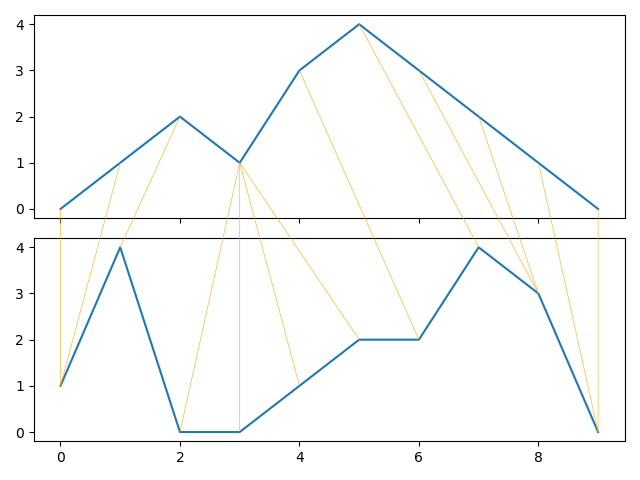
\includegraphics[width=0.7\linewidth]{img/warp}
	\caption{}
	\label{fig:warp}
\end{figure}

\subsection{Matriz de costes locales}
Esta técnica se realiza mediante la comparación de las distancias de todos los pares de puntos en dos secuencias. Una distancia menor implica que estos puntos pueden ser candidatos a ser emparejados. \cite{dwt:dwtdescription}


\subsection{Matriz de costes acumulados}
Una vez emparejados los puntos se usa una matriz de costes acumulados.\cite{s19132882}

En la matriz de costes acumulados se inicializan los valores de la siguiente manera:
\begin{enumerate}
	\item  La primera fila:
	\begin{equation}
		D(1,j) = C(1,j)
	\end{equation}
	\item La primera columna:
	\begin{equation}
		D(i,1) = \sum_{k=1}^{i}C(k,1)
	\end{equation} 
	\item El resto:
	\begin{equation}
		D(i,j) = \min\{D(i-1, j-1),D(i-1,j),D(i,j-1)\} + C(i,j)
	\end{equation}
\end{enumerate}
